\section{Method}

\subsection{Design Objective}

CDS-ASR starts from a speech-to-decision reality: ASR hypotheses increasingly serve as evidence for routing, escalation, conservative review, and abstention. The method turns this reality into a measurable ASR evaluation target: decision stability under plausible transcript alternatives around spoken risk atoms. Transcript-centered metrics describe surface accuracy, semantic-risk metrics describe meaning-level movement, and CDS-ASR adds a consequence-centered layer that measures whether recognition alternatives around decision-critical spoken details move the declared downstream action.

\subsection{Problem Formulation}

Let $x$ denote a speech input, $m$ denote an ASR system, and $\hat{t}_m(x)$ denote the transcript hypothesis produced by $m$. A declared downstream decision function $d(\cdot)$ maps each transcript into an action $a \in \mathcal{A}$, where $\mathcal{A}$ contains routine routing, manual review, priority review, critical escalation, conservative machine action, and abstention. For each hypothesis, CDS-ASR constructs a bounded set of plausible transcript variants $V_m(x)$ around decision-critical spoken details. The model-level score evaluates the strongest action movement induced by these variants, and the row-level score aggregates eligible model hypotheses within the same audio row. This row-clustered formulation keeps the primary case unit aligned with the speech input while preserving model-comparison evidence.

\subsection{CDS-ASR Pipeline}

CDS-ASR has five stages: ASR hypothesis generation, risk-atom extraction, plausible counterfactual variant construction, decision-instability scoring, and aggregate policy replay. Figure~\ref{fig:pipeline} summarizes this pipeline.

\begin{figure}[htbp]
\centering
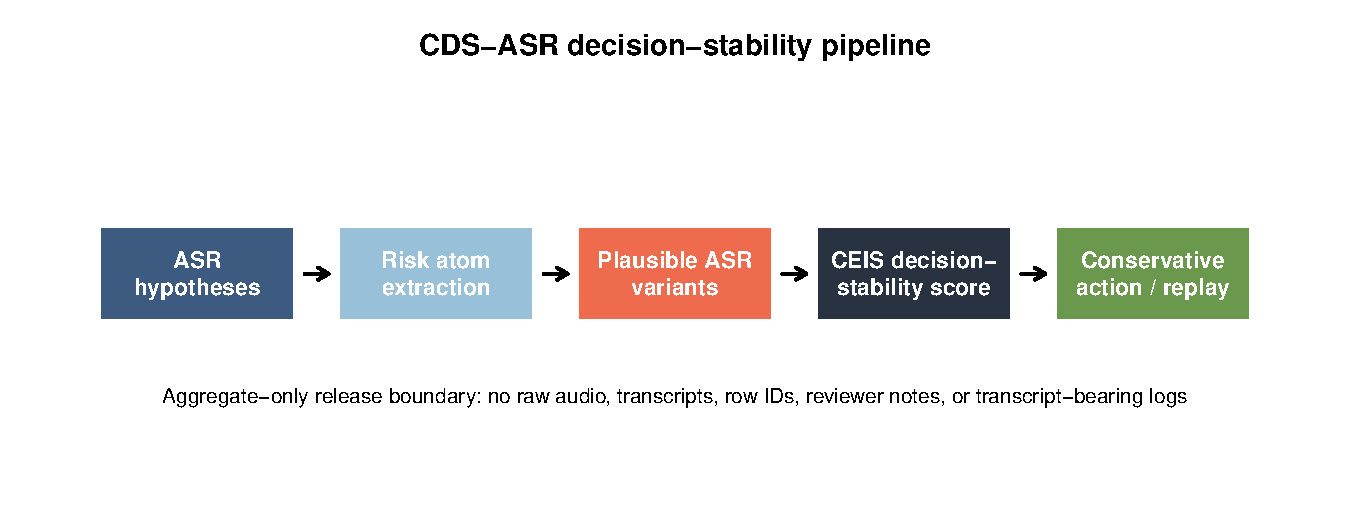
\includegraphics[width=\linewidth]{figures/fig1_pipeline.pdf}
\caption{CDS-ASR decision-stability pipeline. The figure is generated by \artifact{paper_4a_cds_asr/r/build_fig1_pipeline.R} from the manuscript protocol and aggregate method definitions.}
\label{fig:pipeline}
\end{figure}

The pipeline links transcript evidence to action evidence. ASR hypothesis generation creates transcript candidates and runtime signals. Risk-atom extraction identifies spoken spans whose alternatives can move the action boundary. Variant construction creates bounded alternatives from acoustic ambiguity, Mandarin phonetic and lexical confusions, domain-slot alternatives, model disagreement, and quality signals. Decision-instability scoring maps the original hypothesis and each variant through the declared action function. Aggregate policy replay evaluates how conservative operating rules respond to rows with elevated decision-instability evidence.

\subsection{Risk Atom Schema}

Risk atoms are spoken transcript spans that carry a direct decision role. The current schema includes negation, amount, actor, action, time, intent, uncertainty, and scam pattern. These atoms are selected because plausible ASR alternatives around them can move the declared safe action. The paper-facing schema below records the decision role of each atom class. The versioned configuration is \artifact{80_semantic_risk_asr/scoring/ceis_config.json}; the method summary is \artifact{70_experiments/runs/postdoc_evidence_chain_2026_05_25/ceis_method_summary.tsv}.

\begin{center}
\noindent\textbf{Risk atom schema for CDS-ASR.}

\begin{tabularx}{\linewidth}{@{}lL@{}}
\toprule
Risk atom & Decision relevance \\
\midrule
Negation & Can invert whether a transfer, contact, or authorization occurred. \\
Amount & Can change severity, priority, and escalation thresholds. \\
Actor & Can change who initiated or received the action. \\
Action & Can change whether the caller transferred, clicked, paid, reported, or refused. \\
Time & Can change urgency and incident sequence. \\
Intent & Can change whether a phrase is interpreted as request, refusal, uncertainty, or confirmation. \\
Uncertainty & Can change the appropriate review or abstention path. \\
Scam pattern & Can match or miss a known fraud scenario. \\
\bottomrule
\end{tabularx}
\end{center}


\subsection{Counterfactual Variant Contract}

The counterfactual variant contract converts recognition ambiguity into auditable decision-stability evidence. A valid variant is localized around a risk atom or supported by model disagreement and quality signals; it is acoustically or semantically plausible in Mandarin anti-fraud speech; and it is actionable enough to test the declared triage function. The construction draws from Mandarin phonetic and lexical confusions, amount and time slots, actor and action substitutions, negation and uncertainty alternatives, scam-pattern alternatives, and observed ASR disagreement. Public release reports aggregate coverage in \artifact{70_experiments/runs/janus_300_high_stakes_human_audit_selection_2026_05_25/counterfactual_variant_coverage_summary.tsv}.

\subsection{Downstream Decision Function}

The downstream decision function is a declared retrospective policy contract. It maps each transcript and variant to a triage action using the risk atoms visible in the text. The contract turns transcript alternatives into a policy-space representation that supports row-clustered analysis, decision-change labeling, and fixed-budget replay. The action space is operational by design: routine routing, manual review, priority review, critical escalation, conservative machine action, and abstention.

\subsection{CEIS}

CEIS is a bounded decision-instability score over plausible variants:
\[
\mathrm{CEIS}(x) = \max_{v \in V(x)} P_{\mathrm{plaus}}(v \mid x) \cdot W_{\mathrm{atom}}(v) \cdot D(d(\hat{t}), d(v)).
\]
Here $V(x)$ is the set of plausible variants, $P_{\mathrm{plaus}}$ is an audit-bounded plausibility score, $W_{\mathrm{atom}}$ is a risk-atom weight, and $D$ is a downstream decision-distance term. CEIS ranks each row by the strongest plausible movement from transcript evidence to action evidence. The score is interpretable by design: the three terms show why a row is decision-sensitive, which atom carries the action boundary, and how far the declared decision moves.

\subsection{Conservative-Action Policy Contract}

Aggregate policy replay evaluates five operating rules: baseline action, confidence-triggered review, SRES-triggered review, CEIS-triggered conservative action, and CEIS ensemble arbitration. Replay thresholds are retrospective diagnostic operating points on the scoped audit set. The replay layer connects method design to operational use by measuring how transcript accuracy, semantic-risk evidence, and counterfactual decision-stability evidence support conservative review allocation under a fixed budget.
